\newpage 
\section{Trigonometry}\label{sec:Trigonometry}
In this section we review the definitions of trigonometric functions.

\subsection{Angles and Sectors of Circles}
Mathematicians tend to deal mostly with \dfont{radians} and we 
will see later that some formulas are more elegant when using 
radians (rather than degrees). The relationship between degrees 
and radians is:
$$\pi~\mbox{rad}=180^\circ.$$
Using this formula, some common angles can be derived:
$$\begin{array}{|c|c|c|c|c|c|c|c|c|c|c|c|}
\hline
~ & ~ & ~ & ~ & ~ & ~ & ~ & ~ & ~ & ~ & ~ & ~ \\
\mbox{Degrees} & 0^\circ & 30^\circ & 45^\circ & 60^\circ & 90^\circ & 120^\circ & 135^\circ & 150^\circ & 180^\circ & 270^\circ & 360^\circ \\
~ & ~ & ~ & ~ & ~ & ~ & ~ & ~ & ~ & ~ & ~ & ~ \\
\hline
~ & ~ & ~ & ~ & ~ & ~ & ~ & ~ & ~ & ~ & ~ & ~ \\
\mbox{Radians} & 0 & \ds{\frac{\pi}{6}} & \ds{\frac{\pi}{4}} & \ds{\frac{\pi}{3}} & \ds{\frac{\pi}{2}} & \ds{\frac{2\pi}{3}} & \ds{\frac{3\pi}{4}} & \ds{\frac{5\pi}{6}} & \ds{\pi} & \ds{\frac{3\pi}{2}} & 2\pi\\
~ & ~ & ~ & ~ & ~ & ~ & ~ & ~ & ~ & ~ & ~ & ~ \\
\hline
\end{array}$$

\begin{example}{Degrees to Radians}{DegreesToRadians}
To convert $45^\circ$ to radians, multiply by $\ds{\frac{\pi}{180^\circ}}$ to get $\ds{\frac{\pi}{4}}$.
\end{example}

\begin{example}{Radians to Degrees}{RadiansToDegrees}
To convert $\ds{\frac{5\pi}{6}}$ radians to degrees, multiply by $\ds{\frac{180^\circ}{\pi}}$ to get $150^\circ$.
\end{example}

From now on, unless otherwise indicated, we will \ifont{always} use radian measure.

In the diagram below is a sector of a circle with \dfont{central angle} 
$\theta$ and radius $r$ \dfont{subtending} an arc with length $s$.

$$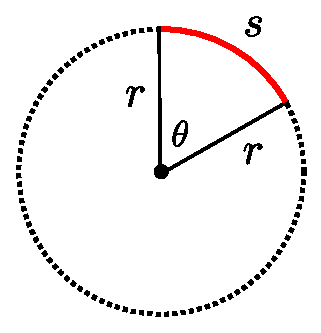
\includegraphics[width=50mm]{images/trig1}$$

When $\theta$ is measure in radians, we have the following 
formula relating $\theta$, $s$ and $r$:
$$\theta=\frac{s}{r}\mbox{\quad~or\quad}s=r\theta.$$

\begin{formulabox}[Sector Area]
The area of the sector is equal to:
$$\mbox{Sector Area}=\frac{1}{2}r^2\theta.$$
\end{formulabox}

\begin{example}{Angle Subtended by Arc}{AngleSubtendedArc}
If a circle has radius $3$ cm, then an angle of $2$ rad is subtended 
by an arc of $6$ cm ($s=r\theta=3\cdot 2=6$).
\end{example}

\begin{example}{Area of Circle}{AreaOfCircle}
If we substitute $\theta=2\pi$ (a complete revolution) into the sector 
area formula we get the area of a circle: 
$$A=\frac{1}{2}r^2(2\pi)=\pi r^2.$$
\end{example}
\subsection{Trigonometric Functions}
There are six basic trigonometric functions:
\begin{multicols}{2}
\begin{itemize}
	\item Sine (abbreviated by $\sin$)
	\item Cosine (abbreviated by $\cos$)
	\item Tangent (abbreviated by $\tan$)
	\item Cosecant (abbreviated by $\csc$)
	\item Secant (abbreviated by $\sec$)
	\item Cotangent (abbreviated by $\cot$)
\end{itemize}
\end{multicols}

We first describe trigonometric functions in terms of ratios of two sides of a \ifont{right angle triangle} containing the angle $\theta$. 

$$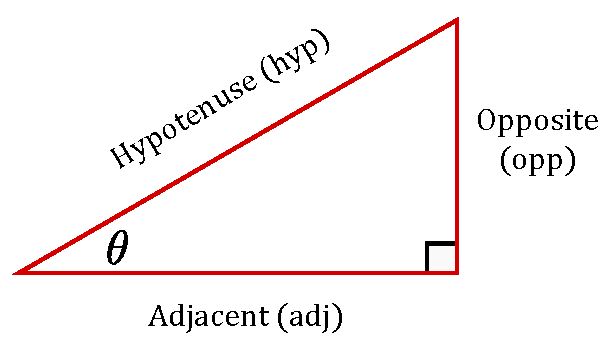
\includegraphics[width=2.5in]{images/trig2}$$

With reference to the above triangle, for an acute angle $\theta$ (that is, $0\leq\theta<\pi/2$), the six trigonometric functions can be described as follows:
$$\begin{array}{ccc}
\ds\sin\theta=\frac{\rm opp}{\rm hyp}&\qquad&\ds\csc\theta=\frac{\rm hyp}{\rm opp}\\
\\
\ds\cos\theta=\frac{\rm adj}{\rm hyp}&\qquad&\ds\sec\theta=\frac{\rm hyp}{\rm adj}\\
\\
\ds\tan\theta=\frac{\rm opp}{\rm adj}&\qquad&\ds\cot\theta=\frac{\rm adj}{\rm opp}\\
\end{array}$$

\begin{formulabox}[Mnemonic]
The mnemonic \ifont{SOH CAH TOA} is useful in remembering how trigonometric functions of acute angles relate to the sides of a right triangle.
\end{formulabox}

This description does not apply to \ifont{obtuse} or \ifont{negative angles}.
To define the six basic trigonometric functions we first define sine and cosine as the lengths of various line segments from a unit circle, and then we define the remaining four basic trigonometric functions in terms of sine and cosine.

Take a line originating at the origin (making an angle of $\theta$ with the positive half of the $x$-axis) and suppose this line intersects the unit circle at the point $(x,y)$.
The $x$- and $y$-coordinates of this point of intersection are equal to $\cos\theta$ and $\sin\theta$, respectively.
$$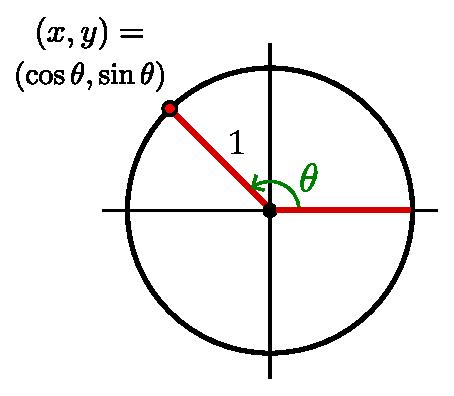
\includegraphics[width=2.3in]{images/trig3}$$
For angles greater than $2\pi$ or less than $-2\pi$, simply continue to rotate around the circle.
In this way, sine and cosine become periodic functions with period $2\pi$:
$$\sin\theta = \sin\left(\theta + 2\pi k \right)\qquad\qquad \cos\theta = \cos\left(\theta + 2\pi k \right)$$
for any angle $\theta$ and any integer $k$.

Above, only sine and cosine were defined directly by the circle.
We now define the remaining four basic trigonometric functions in terms of the functions $\sin\theta$ and $\cos\theta$:
$$\tan\theta = \frac{\sin\theta}{\cos\theta} \qquad \sec\theta = \frac{1}{\cos\theta} \qquad \csc\theta = \frac{1}{\sin\theta} \qquad \cot\theta = \frac{\cos\theta}{\sin\theta}$$
\subsection{Computing Exact Trigonometric Ratios}
The \dfont{unit circle} is often used to determine the \ifont{exact} value of a particular trigonometric function.

$$
\includegraphics[width=5in]{images/unit-circle}$$

Reading from the unit circle one can see that $\cos (5\pi/6)=-\sqrt 3/2$ and $\sin (5\pi/6)=1/2$ (remember that the $x\,$-coordinate is $\cos\theta$ and the $y$-coordinate is $\sin\theta$ for the unit circle).
However, we don't always have access to the unit circle.
In this case, we can compute the exact trigonometric ratios for $\theta=5\pi/6$ by using \dfont{special triangles} and the \dfont{CAST rule} described below.

The first special triangle has angles of $45^\circ,45^\circ,90^\circ$ (i.e., $\pi/4,\pi/4,\pi/2$) with side lengths $1,1,\sqrt 2$, while the second special triangle has angles of $30^\circ,60^\circ,90^\circ$ (i.e., $\pi/6,\pi/3,\pi/2$) with side lengths $1,2,\sqrt 3$. They are classically referred to as the $1-1-\sqrt{2}$ triangle, and the $1-2-\sqrt{3}$ triangle, respectively, shown below.
$$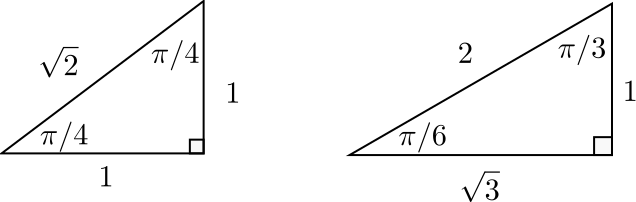
\includegraphics[width=4.0in]{images/trig4}$$

\begin{formulabox}[Mnemonic]
The first triangle should be easy to remember. 
To remember the second triangle, place the largest number ($2$) across from the largest angle ($90^\circ=\pi/2$).
Place the smallest number ($1$) across from the smallest angle ($30^\circ=\pi/6$).
Place the middle number ($\sqrt 3\approx 1.73$) across from the middle angle ($60^\circ=\pi/3$).
Double check using the Pythagorean Theorem that the sides satisfy $a^2+b^2=c^2$.
\end{formulabox}

The special triangles allow us to compute the exact value (excluding the sign) of trigonometric ratios, but to determine the sign, we can use the \ifont{CAST rule}.

\begin{formulabox}[The CAST Rule]
The CAST rule says that in quadrant I all three of $\sin\theta$, $\cos\theta$, $\tan\theta$ are positive.
In quadrant II, only $\sin\theta$ is positive, while $\cos\theta$, $\tan\theta$ are negative.
In quadrant III, only $\tan\theta$ is positive, while $\sin\theta$, $\cos\theta$ are negative.
In quadrant IV, only $\cos\theta$ is positive, while $\sin\theta$, $\tan\theta$ are negative. 
To remember this, simply label the quadrants by the letters C-A-S-T starting in the bottom right and labelling counter-clockwise.
\end{formulabox} 

$$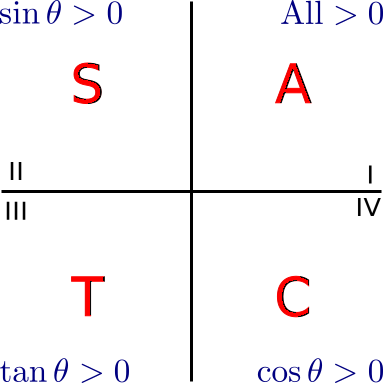
\includegraphics[width=2.5in]{images/trig5}$$

\begin{example}{Determining Trigonometric Ratios Without Unit Circle}{CASTRule}
Determine $\sin (5\pi/6)$, $\cos (5\pi/6)$, $\tan (5\pi/6)$, $\sec (5\pi/6)$, $\csc (5\pi/6)$ and $\cot (5\pi/6)$ exactly by using the special triangles and CAST rule.
\end{example}

\begin{solution} 
We start by drawing the $xy$-plane and indicating our angle of $5\pi/6$ in standard position (positive angles rotate \ifont{counterclockwise} while negative angles rotate \ifont{clockwise}).
Next, we drop a perpendicular to the $x\,$-axis (never drop it to the $y$-axis!).
$$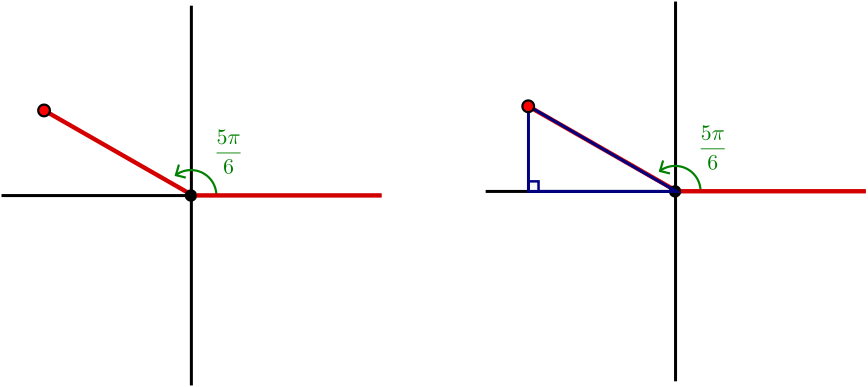
\includegraphics[width=4in]{images/trig6}$$
Notice that we can now figure out the angles in the triangle.
Since $180^\circ=\pi$, we have an interior angle of $\pi-5\pi/6=\pi/6$ inside the triangle. 
As the \ifont{angles of a triangle add up to $180^\circ=\pi$}, the other angle must be $\pi/3$. 
This gives one of our special triangles.
We label it accordingly and add the CAST rule to our diagram.
$$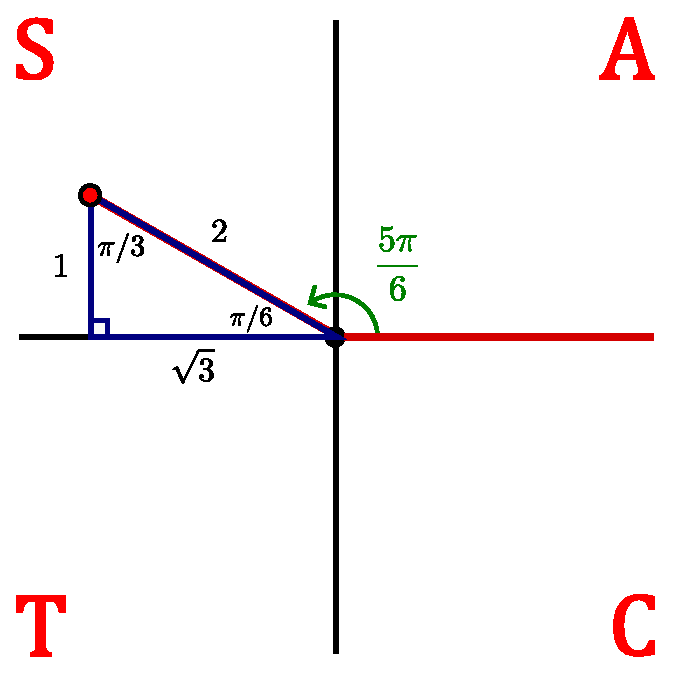
\includegraphics[width=3in]{images/trig7}$$
From the above figure we see that $5\pi/6$ lies in quadrant II where $\sin\theta$ is positive and $\cos\theta$ and $\tan\theta$ are negative.
This gives us the \ifont{sign} of $\sin\theta$, $\cos\theta$ and $\tan\theta$.
To determine the \ifont{value} we use the special triangle and SOH CAH TOA.

Using $\sin\theta=opp/hyp$ we find a value of $1/2$.
But $\sin\theta$ is positive in quadrant II, therefore, 
$$\sin \left(\frac{5\pi}{6}\right)=\frac{1}{2}.$$

Using $\cos\theta=adj/hyp$ we find a value of $\sqrt 3/2$.
But $\cos\theta$ is negative in quadrant II, therefore, 
$$\cos \left(\frac{5\pi}{6}\right) =-\frac{\sqrt 3}{2}.$$

Using $\tan\theta=opp/adj$ we find a value of $1/\sqrt 3$.
But $\tan\theta$ is negative in quadrant II, therefore, 
$$\tan \left(\frac{5\pi}{6}\right) =-\frac{1}{\sqrt 3}.$$

To determine $\sec\theta$, $\csc\theta$ and $\cot\theta$ we use the definitions:
$$\csc \left(\frac{5\pi}{6}\right)  = \ds\frac{1}{\sin \left(\frac{5\pi}{6}\right)}  = 2,
\qquad \sec \left(\frac{5\pi}{6}\right)  = \ds\frac{1}{\cos \left(\frac{5\pi}{6}\right) } = -\frac{2}{\sqrt 3},
\qquad\cot \left(\frac{5\pi}{6}\right) = \ds\frac{1}{\tan \left(\frac{5\pi}{6}\right)} = -\sqrt 3.$$
\end{solution}

\begin{example}{CAST Rule}{CASTRule2}
If $\cos\theta=3/7$ and $3\pi/2<\theta< 2\pi$, then find $\cot\theta$.
\end{example}

\begin{solution} 
We first draw a right angle triangle.
Since $\cos\theta=adj/hyp=3/7$, we let the adjacent side have length $3$ and the hypotenuse have length $7$.
$$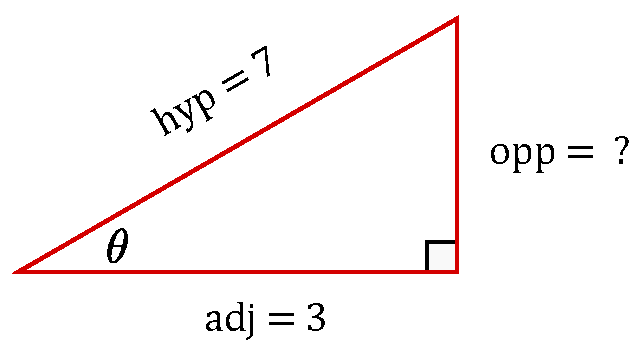
\includegraphics[height=1.1in]{images/trig8}$$
Using the Pythagorean Theorem, we have $3^2+(\mbox{opp})^2=7^2$.
Thus, the opposite side has length $\sqrt{40}$.
$$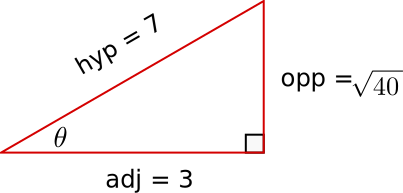
\includegraphics[height=1.1in]{images/trig9}$$
%Recall that \green{right angle triangles} can give us the \red{value} of trigonometric ratios while the \green{CAST rule} gives us the \red{sign}.**
To find $\cot\theta$ we use the definition:
$$\cot\theta=\frac{1}{\tan\theta}.$$
Since we are given $3\pi/2<\theta< 2\pi$, we are in the fourth quadrant. By the CAST rule, $\tan\theta$ is negative in this quadrant.
As $\tan\theta=opp/adj$, it has a value of $\sqrt{40}/3$, but by the CAST rule it is negative, that is,
$$\tan\theta=-\frac{\sqrt{40}}{3}.$$
Therefore,
$$\cot\theta=-\frac{3}{\sqrt{40}}.$$
\end{solution}
\subsection{Graphs of Trigonometric Functions}
The graph of the functions $\sin x$ and $\cos x$ can be visually represented as:

$$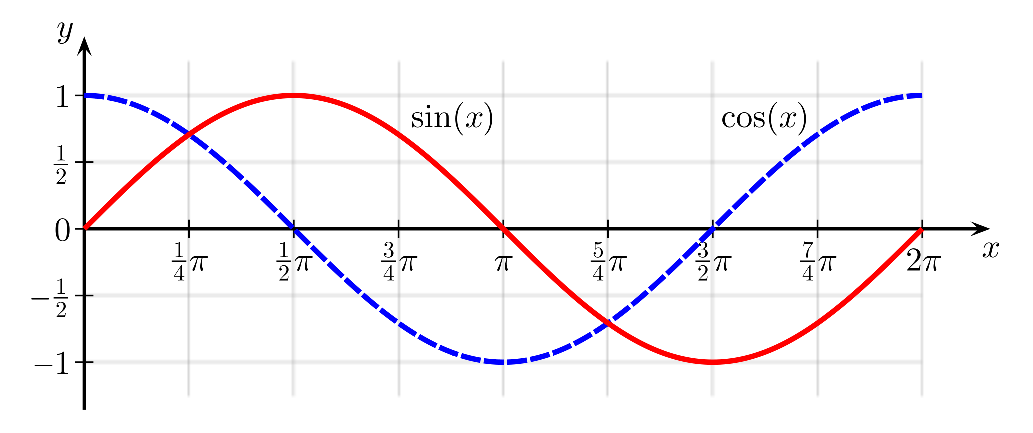
\includegraphics[width=4.0in]{images/sine-cosine}$$

Both $\sin x$ and $\cos x$ have domain $(-\infty,\infty)$ and range $[-1,1]$.
That is,
$$-1\leq\sin x\leq 1\qquad -1\leq\cos x\leq 1.$$
The zeros of $\sin x$ occur at the integer multiples of $\pi$, that is, $\sin x=0$ whenever $x=n\pi$, where $n$ is an integer.
Similarly, $\cos x=0$ whenever $x=\pi/2+n\pi$, where $n$ is an integer.

The six basic trigonometric functions can be visually represented as:

$$\includegraphics[width=7in]{images/trig-functions-new}$$

Both tangent and cotangent have range $(-\infty,\infty)$, whereas cosecant and secant have range $(-\infty,-1]\cup[1,\infty)$.
Each of these functions is periodic. Tangent and cotangent have period $\pi$, whereas sine, cosine, cosecant and secant have period $2\pi$.
\subsection{Trigonometric Identities}
There are numerous trigonometric identities, including those relating to shift/periodicity, Pythagoras type identities, double-angle formulas, half-angle formulas and addition formulas.
We list these below.

\begin{enumerate}
\item[1.] \dfont{Shifts and periodicity}
$$\begin{array}{|rcl|rcl|rcl|}
\hline
~&~&~&~&~&~&~&~&~\\
\ds{\sin (\theta + 2\pi)} & = & \ds{\sin \theta} &
\ds{\cos (\theta + 2\pi)} &= & \ds{\cos \theta} &
\ds{\tan (\theta + 2\pi)} &= & \ds{\tan \theta} \\
~&~&~&~&~&~&~&~&~\\
\hline
~&~&~&~&~&~&~&~&~\\
\ds{\sin (\theta + \pi)} &= & \ds{-\sin \theta} &
\ds{\cos (\theta + \pi)} &= & \ds{-\cos \theta} &
\ds{\tan (\theta + \pi)} &= & \ds{\tan \theta} \\
~&~&~&~&~&~&~&~&~\\
\hline
~&~&~&~&~&~&~&~&~\\
\ds{\sin (-\theta)} &= & \ds{-\sin \theta} & 
\ds{\cos (-\theta)} &= & \ds{\cos \theta} & 
\ds{\tan (-\theta)} &= & \ds{-\tan \theta}  \\
~&~&~&~&~&~&~&~&~\\
\hline
~&~&~&~&~&~&~&~&~\\
\ds{\sin \left(\theta +\frac{\pi}{2}\right) } &= &  \ds{\cos \theta} &
\ds{\cos \left(\theta -\frac{\pi}{2}\right)} &= &  \ds{\sin \theta} &
\ds{\tan \left(\frac{\pi}{2}-\theta\right)} &= & \ds{\cot \theta}  \\
~&~&~&~&~&~&~&~&~\\
\hline
\end{array}$$
\end{enumerate}

\begin{multicols}{2}
\begin{enumerate}
\item[2.] \dfont{Pythagoras type formulas}

$ \begin{array}{|rcl|} \hline	
&& \\
\ds{\sin ^2 \theta + \cos ^2 \theta} & = & \ds{1}\\
&& \\
\ds{\tan^2 \theta + 1} & = & \ds{\sec^2 \theta} \\
&& \\
\ds{1 + \cot ^2 \theta}  & = & \ds{\csc^2 \theta} \\
&& \\ \hline
\end{array} $

\vspace{5mm} 
\item[3.] \dfont{Addition and subtraction formulas}

$\begin{array}{|rcl|} \hline
&& \\	
\ds{\sin(\theta+\phi)} & = & \ds{\sin\theta\cos\phi + \cos\theta\sin\phi} \\
&& \\
\ds{\cos(\theta+\phi)} & = & \ds{\cos\theta\cos\phi - \sin\theta\sin\phi} \\
&& \\
\ds{\tan(\theta+\phi)} & = & \ds{\frac{\tan\theta + \tan\phi}{1 - \tan\theta\tan\phi}}\\
&& \\
\ds{\sin(\theta-\phi)} & = & \ds{\sin\theta\cos\phi - \cos\theta\sin\phi} \\
&& \\
\ds{\cos(\theta-\phi)} & = & \ds{\cos\theta\cos\phi + \sin\theta\sin\phi} \\
&& \\ \hline 
\end{array} $


\item[4.] \dfont{Double-angle formulas}

$\begin{array}{|rcl|} \hline
&& \\	
\ds{\sin(2\theta)} & =  & \ds{2\sin\theta\cos\theta} \\
&& \\
\ds{\cos(2\theta)} & = & \ds{\cos^2\theta - \sin^2\theta}\\
& =  & \ds{2\cos^2\theta - 1} \\
& = & \ds{1-2\sin^2\theta}\\
&& \\ \hline 
\end{array}$

\vspace{4mm} 
\item[5.] \dfont{Half-angle formulas}

$ \begin{array}{|rcl|} \hline 
&& \\
\ds{\cos^2\theta} & = & \ds{\frac{1+\cos(2\theta)}{2}} \\
&& \\
\ds{\sin^2\theta} & = & \ds{\frac{1-\cos(2\theta)}{2}} \\
&& \\ \hline 
\end{array} $

\end{enumerate}
\end{multicols}

\begin{example}{Double Angle}{DoubleAngle}
Find all values of $x$ with $0\leq x\leq \pi$ such that $\sin 2x=\sin x$.
\end{example}

\begin{solution} 
Using the double-angle formula $\sin 2x = 2\sin x \cos x$ we have:

\hspace{3cm} $$\begin{array}{rcl}
\ds{2\sin x\cos x} & = & \ds{\sin x} \\
\ds{2\sin x\cos x- \sin x} & = & \ds{0} \\
\ds{\sin x \, (2\cos x - 1)} & = & \ds{0} \\
\end{array}$$

Thus, either \hspace{1cm} $\,\, \sin x=0 \,\, $ or $\,\, \cos x = 1/2\,\, $. \\

For the first case when $\,\, \sin x = 0 \,\, $, we get $\, x=0 \, $ or $\, x=\pi \,$.
For the second case when $\,\,\cos x = 1/2 \,\,$, we get $\, x=\pi/3 \,$ (use the special triangles and CAST rule to get this).
Thus, we have three solutions: $x=0, \, \pi/3, \, \pi$.
\end{solution}

%%%%%%%%%%%%%%%%%%%%%%%%%%%%%%%%%%%%%%%%%%%%

\Opensolutionfile{solutions}[ex]
\section*{Exercises for \ref{sec:Trigonometry}}

\begin{enumialphparenastyle}

%\vfill\null
%\columnbreak

\begin{multicols}{2}
%%%%%%%%%%
\begin{ex}
Convert from degrees to radians.\\
$\begin{array}{cccc}
(a) \hspace{1mm} 90^{\circ} & (b) \hspace{1mm} 135^{\circ} & (c) \hspace{1mm} 210^{\circ} & (d) \hspace{1mm} 300^{\circ} 
\end{array}$  
\begin{sol}
$\begin{array}{cccc}
	(a) \hspace{1mm} \pi/2 & (b) \hspace{1mm} 3\pi/4 & (c) \hspace{1mm} 7\pi/6 & (d) \hspace{1mm} 5\pi/3 
\end{array}$  
\end{sol}
\end{ex}

\begin{ex}
	Convert from radians to degrees.\\
	$\begin{array}{cccc}
	(a) \hspace{1mm} \ds{\frac{\pi}{3}} & (b) \hspace{1mm} \ds{\frac{7\pi}{12}} & (c) \hspace{1mm} \ds{\frac{3\pi}{2}} & (d) \hspace{1mm} \ds{\frac{-5\pi}{12}} 
	\end{array}$  
\begin{sol}
	$\begin{array}{cccc}
	(a) \hspace{1mm} 60^{\circ} & (b) \hspace{1mm} 105^{\circ} & (c) \hspace{1mm} 270^{\circ} & (d) \hspace{1mm} 285^{\circ} 
	\end{array}$   
\end{sol}
\end{ex}

\begin{ex}
	If a circle has radius $5 \,\, cm$, find the length of arc subtended by a central angle of $\pi /6$.
\end{ex}
\begin{sol} 
	$\ds{5\pi/6 \,\, cm}$
\end{sol}

\begin{ex}
	Find the radius of a circular sector with angle $\pi /4 $ and arc length $2\pi \,\, cm$.
\begin{sol}
	$8 \,\,cm$
\end{sol}
\end{ex} 

%%%%%%%%%%
\begin{ex} 
	Compute the following:
	\begin{multicols}{2}
		\begin{enumerate}
			\item	$\sin(3\pi)$
			\item	$\sec(5\pi / 6)$
			\item	$\cos(-\pi / 3)$
			\item	$\csc(4\pi / 3)$
			\item	$\tan(7\pi / 4)$
			\item	$\cot(13\pi  /4)$
		\end{enumerate}
	\end{multicols}
\begin{sol}
  $\begin{array}{llllll}
  (a) $0$ & (b) $-2\sqrt{3}/3$ & (c) $1/2$ & (d) $-2\sqrt{3}/3$ & (e) $-1$ & (f) $1$	 
\end{array}$
\end{sol}	 
\end{ex}	 	 
	
\begin{ex}
If $\ds{\cos \theta =\frac{2}{5}}$ and $0 <\theta <\pi/2$, find the other five trigonometric functions of $\theta$.
\begin{sol}
	$\ds{\sin \theta = \frac{\sqrt{21}}{5} ; \hspace{4mm} \tan \theta = \frac{\sqrt{21}}{2} ; \hspace{4mm} \csc \theta = \frac{5}{\sqrt{21}} ; \hspace{4mm} \sec \theta = \frac{5}{2} ; \hspace{4mm} \cot \theta = \frac{2}{\sqrt{21}}  }$		
\end{sol}
\end{ex}
	
\begin{ex}
Find all values of $\theta$ that satisfy the equation. Express your answer in radians.\\
$\begin{array}{ll}
(a) \hspace{1mm} \sin \theta = -1 & (b) \hspace{1mm}  \cos 2\theta = 1/2
\end{array}$
\begin{sol}
(a) $2n\pi-\pi/2$, any integer $n$; (b) $n\pi\pm\pi/6$, any integer $n$
\end{sol}
\end{ex}


%%%%%%%%%%
\begin{ex}
If $\sin\theta=\frac{3}{5}$ and $\frac{\pi}{2}<\theta<\pi$, then find $\sec\theta$.
\begin{sol}
$-\frac{5}{4}$
\end{sol}
\end{ex}

%%%%%%%%%%
\begin{ex}
Suppose that $\tan\theta=x$ and $\pi<\theta<\frac{3\pi}{2}$, find $\sin\theta$ and $\cos\theta$ in terms of $x$.
\begin{sol}
$\sin\theta=-x/\sqrt{x^{2}+1}$, $\cos\theta=-1/\sqrt{x^{2}+1}$.
\end{sol}
\end{ex}

%%%%%%%%%%
\begin{ex}
Find an angle $\theta$ such that $-\frac{\pi}{2}<\theta<\frac{\pi}{2}$ and $\sin\theta=\sin\frac{23\pi}{7}$.
\begin{sol}
$-\frac{2\pi}{7}$ is the unique answer.
\end{sol}
\end{ex}


%%%%%%%%%%
\begin{ex} 
Use an angle sum identity to compute the following. \\

\vspace{-2mm} \hspace{4mm}  (a) \hspace{1mm} $\cos(\pi/12)$ \hspace{1cm} (b) \hspace{1mm} $\tan(5\pi/12)$
\begin{sol} 
(a) $(\sqrt{2}+\sqrt{6})/4$; \hspace{1cm} (b) $-(1+\sqrt3)/(1-\sqrt3)=2+\sqrt3$
\end{sol}
\end{ex}


%%%%%%%%%%
\begin{ex} Sketch the following functions:
	\begin{multicols}{2}
		\begin{enumerate}
			\item	$y=2\sin x$
			\item	$y=\sin 3x$
			\item	$y=\sin(-x)$
			\item   $\ds{y=\cos \left(x-\frac{\pi}{3} \right)}$
			\item   $y=|\sin x|$ 
			\item   $\ds{y=2+\sin \left(x+\frac{\pi}{4} \right)}$
		\end{enumerate}
	\end{multicols}
\end{ex}

%%%%%%%%%%
\begin{ex} Verify the following identities
 \begin{enumerate}
	\item	$\ds{\frac{\cos^2 t }{1-\sin t } = 1+\sin t }$
	\item	$\ds{2\csc 2\theta=\sec \theta \csc \theta} $
	\item	$\ds{\sin 3\theta - \sin \theta  = 2\cos 2\theta\sin \theta}$
\end{enumerate}
\end{ex}



%%%%%%%%%%
\begin{ex} Find all values of $x$ in the interval $[0, \, 2\pi]$ that satisfy the equation.\\
\begin{multicols}{2}
	\begin{enumerate}
		\item $\ds{\sin 2x =1}$ 
	    \item $\ds{\sin x = \tan x}$
	    \item $\ds{\cos x = \sin 2x}$ 
	    \item $\ds{2\cos x + 1 =0}$
	     \item $\ds{2\sin x -1 -\sin^2 x = 0}$ 
	 \end{enumerate}
\end{multicols}	 
\begin{sol}
 (a)  (b) (c) (d) (e) $t=\pi/2$
\end{sol}
\end{ex}

\end{multicols}

\end{enumialphparenastyle}
